% This is text associated with the open textbook "Open Electromagnetics"
% See immediately below for author, date
% This work is licensed under the Creative Commons Attribution-ShareAlike 4.0 International License. (CC BY-SA 4.0) 
% To view a copy of the license, visit http://creativecommons.org/licenses/by-sa/4.0/

%ORB TITLE Microstrip Line
%ORB AUTHOR 0        # S.W. Ellingson, Virginia Tech (ellingson@vt.edu)
%ORB DATE 20180802   # yyyymmdd
%ORB ABSTRACT Basics of microstrip lines in terms of elementary transmission line theory 

\label{m0082_Microstrip_Line} % <-- Must match name of this file and module directory name.  Don't mess with this!
\index{microstrip|(}
\index{transmission line!microstrip|see{microstrip}}

A microstrip transmission line consists of a narrow metallic trace separated from a metallic ground plane by a slab of dielectric material, as shown in Figure~\ref{m0082_fMicrostripCrossSection}. 
This is a natural way to implement a transmission line on a printed circuit board,
\index{printed circuit board (PCB)}
and so accounts for an important and expansive range of applications.
The reader should be aware that microstrip is distinct from \emph{stripline},
\index{stripline}
\index{transmission line!stripline}
which is a very different type of transmission line; see ``Additional Reading'' at the end of this section for disambiguation of these terms.
%
\begin{figure}
\begin{center}
\pdftooltip{{  % note double braces
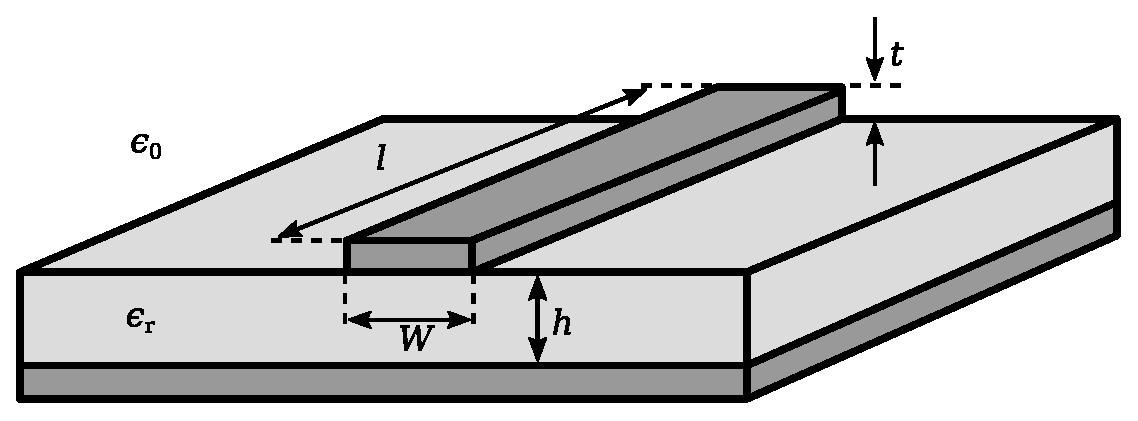
\includegraphics[width=\columnwidth]{modules/m0082_fMicrostripCrossSection.eps}
% https://commons.wikimedia.org/wiki/File:Microstrip_scheme.svg
}}{A diagram of a microstrip transmission line. Certain dimensions are labeled: Length of the metal trace (l), width of the metal trace (W), thickness of the metal trace (t), and height of the dielectric slab (h). Epsilon sub r is labeled on the dielectric and epsilon sub 0 is labeled on the space next to the microstrip transmission line.}
\end{center} 
\centerline{\scriptsize 
\copyright~\hyperref[m0082_fMicrostripCrossSection_Credit]{7head7metal7}  
\href{https://creativecommons.org/licenses/by-sa/3.0/}{CC BY~SA 3.0} 
(modified)
} 
\caption{
\label{m0082_fMicrostripCrossSection}
Microstrip transmission line structure and design parameters.
}
\end{figure}

A microstrip line is single-ended\footnote{The reference in ``Additional Reading'' at the end of this section may be helpful if you are not familiar with this concept.} in the sense that the conductor geometry is asymmetric and the one conductor -- namely, the ground plane -- also normally serves as ground for the source and load.

The spacer material is typically a low-loss dielectric 
\index{dielectric (material)}
material having permeability approximately equal to that of free space ($\mu \approx \mu_0$) and relative permittivity $\epsilon_r$ in the range 2 to about 10 or so.

A microstrip line nominally exhibits TEM 
\index{transmission line!transverse electromagnetic (TEM)}
field structure.
This structure is shown in Figure~\ref{m0082_fMicrostripFieldStructure}.
Note that electric and magnetic fields exist both in the dielectric and in the space above the dielectric, which is typically (but not always) air. 
This complex field structure makes it difficult to describe microstrip line concisely in terms of the equivalent circuit parameters of the lumped-element model.  
Instead, expressions for $Z_0$ directly in terms of $h/W$ and $\epsilon_r$ are typically used instead.  
A variety of these expressions are in common use, representing different approximations and simplifications.  
A widely-accepted and broadly-applicable expression is:\footnote{This is from Wheeler 1977, cited in ``Additional Reading'' at the end of this section.}
%
\begin{equation}
\begin{split}
Z_0 & \approx \frac{42.4~\Omega}{\sqrt{\epsilon_r+1}} ~\times \\
    &
\ln\left[
    1 +
    \frac{4h}{W'}
    \left( \Phi + \sqrt{ \Phi^2 + \frac{1+1/\epsilon_r}{2}\pi^2 } \right)
   \right]
\end{split}
\label{m0082_eWheeler10}
\end{equation}
% 
where
%
\begin{equation}
\Phi \triangleq \frac{ 14 + 8/\epsilon_r }{ 11 } \left( \frac{4h}{W'} \right)
\end{equation}
%
and $W'$ is $W$ adjusted to account for the thickness $t$ of the microstrip line.  Typically $t\ll W$ and $t \ll h$, for which $W'\approx W$.  
Simpler approximations for $Z_0$ are also commonly employed in the design and analysis of microstrip lines. 
These expressions are limited in the range of $h/W$ for which they are valid, and can usually be shown to be special cases or approximations of Equation~\ref{m0082_eWheeler10}.
Nevertheless, they are sometimes useful for quick ``back of the envelope'' calculations.
%
\begin{figure}
\begin{center}
\pdftooltip{{  % note double braces
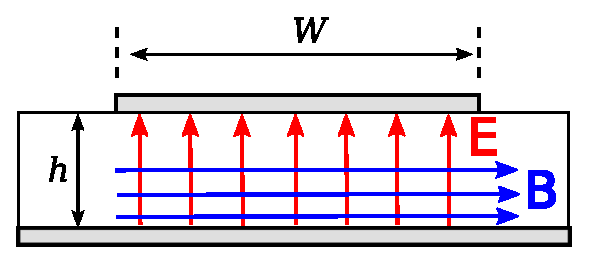
\includegraphics[width=2.5in]{modules/m0082_fMicrostripFieldStructure.eps}
}}{A cross-sectional view of the microstrip transition line. The electric field, "E", is represented by a row of red parallel arrows pointing vertically from the ground plane to the metallic trace.The magnetic field, "B", is represented by parallel blue arrows perpendicular to the electric field arrows, pointing to the right.}
\end{center} 
\caption{\label{m0082_fMicrostripFieldStructure}Structure of the electric and magnetic fields within microstrip line. (The fields \emph{outside} the line are possibly significant, complicated, and not shown.)  In this case, the wave is propagating away from the viewer.}
\end{figure}

Accurate expressions for wavelength $\lambda$, phase propagation constant $\beta$, and phase velocity $v_p$ are similarly difficult to obtain for waves in microstrip line.
An approximate technique employs a result from the theory of uniform plane waves in unbounded media (Equation~\ref{m0036_eBetaDef} from Section~\ref{m0036_Wave_Equations_SourceFree_Lossless}):
%
\begin{equation}
\beta = \omega\sqrt{\mu\epsilon}
\end{equation}
%
It turns out that the electromagnetic field structure in the space between the conductors is well-approximated as that of a uniform plane wave in unbounded media having the same permeability $\mu_0$ but a different relative permittivity, which we shall assign the symbol $\epsilon_{r,eff}$ (for ``\emph{effective} relative permittivity''). 
\index{permittivity!effective}
Then
%
\begin{flalign}
\beta &\approx \omega\sqrt{\mu_0~\epsilon_{r,eff}~\epsilon_0} ~~~\mbox{(low-loss microstrip)} \nonumber \\
      &=\beta_0 \sqrt{\epsilon_{r,eff}}
\end{flalign}
%
In other words, the phase propagation constant in a microstrip line can be approximated as the free-space phase propagation $\beta_0\triangleq\omega\sqrt{\mu_0\epsilon_0}$ times a correction factor $\sqrt{\epsilon_{r,eff}}$. 
Then $\epsilon_{r,eff}$ may be crudely approximated as follows:
%
\begin{equation}
\epsilon_{r,eff} \approx \frac{\epsilon_r+1}{2}
\end{equation}
%
i.e., $\epsilon_{r,eff}$ is roughly the average of the relative permittivity of the dielectric slab and the relative permittivity of free space.  
The assumption employed here is that $\epsilon_{r,eff}$ is approximately the average of these values because some fraction of the power in the guided wave is in the dielectric, and the rest is above the dielectric.
Various approximations are available to improve on this approximation; however, in practice variations in the value of $\epsilon_r$ for the dielectric due to manufacturing processes typically make a more precise estimate irrelevant.

Using this concept, we obtain
%
\begin{equation}
\lambda = \frac{2\pi}{\beta} = \frac{2\pi}{\beta_0\sqrt{\epsilon_{r,eff}}} = \frac{\lambda_0}{\sqrt{\epsilon_{r,eff}}}
\end{equation}
%
where $\lambda_0$ is the free-space wavelength
\index{wavelength!in microstrip}
$c/f$.
Similarly the phase velocity 
\index{phase velocity!in microstrip}
$v_p$, can be estimated using the relationship
%
\begin{equation}
v_p = \frac{\omega}{\beta} = \frac{c}{\sqrt{\epsilon_{r,eff}}}
\end{equation}
%
i.e., the phase velocity in microstrip is slower than $c$ by a factor of $\sqrt{\epsilon_{r,eff}}$.

%ORB EXAMPLE
~\\ \begin{example} 
\begin{mdframed}[backgroundcolor=brown!20,linecolor=brown!20]\raggedright
$50~\Omega$ Microstrip in FR4 
\index{FR4}
Printed Circuit Boards.
\index{printed circuit board (PCB)}
\\~\\
FR4 is a low-loss fiberglass epoxy dielectric that is commonly used to make printed circuit boards (see ``Additional Reading'' at the end of this section).
FR4 circuit board material is commonly sold in a slab having thickness $h\cong 1.575$~mm 
%(62~mils) 
with $\epsilon_r\cong 4.5$.  
Let us consider how we might implement a microstrip line having $Z_0=50~\Omega$ using this material.
Since $h$ and $\epsilon_r$ are fixed, the only parameter remaining to set $Z_0$ is $W$.
A bit of experimentation with Equation~\ref{m0082_eWheeler10} reveals that $h/W\approx 1/2$ yields $Z_0\approx 50~\Omega$ for $\epsilon_r=4.5$.  
Thus, $W$ should be about 3.15~mm.
The effective relative permittivity is 
%
\begin{equation}
\epsilon_{r,eff}\approx(4.5+1)/2 = 2.75
\nonumber
\end{equation}
%
so the phase velocity for the wave guided by this line is about $c/\sqrt{2.75}$; i.e., 60\% of $c$.
Similarly, the wavelength of this wave is about 60\% of the free space wavelength.
\end{mdframed}\end{example}

%------------------------------------

{\bf Additional Reading:}
\begin{itemize}
\item ``\href{https://en.wikipedia.org/wiki/Microstrip}{Microstrip}'' on Wikipedia.
\item ``\href{https://en.wikipedia.org/wiki/Printed_circuit_board}{Printed circuit board}'' on Wikipedia.
\item ``\href{https://en.wikipedia.org/wiki/Stripline}{Stripline}'' on Wikipedia.
\item ``\href{https://en.wikipedia.org/wiki/Single-ended_signaling}{Single-ended signaling}'' on Wikipedia.
\item Sec.~8.7 (``Differential Circuits'') in S.W.~Ellingson, \emph{Radio Systems Engineering}, Cambridge Univ.\ Press, 2016. 
\item H.A.\ Wheeler, ``Transmission Line Properties of a Strip on a Dielectric Sheet on a Plane,'' {\it IEEE Trans.\ Microwave Theory \& Techniques}, Vol.~25, No.~8, Aug~1977, pp.~631--47. % http://dx.doi.org/10.1109/TMTT.1977.1129179.
\item ``\href{https://en.wikipedia.org/wiki/FR-4}{FR-4}'' on Wikipedia.
\end{itemize}
 
\index{microstrip|)}

